\documentclass[11pt]{article}

\usepackage[margin=1in]{geometry}
\usepackage{amsmath}
\usepackage{amssymb}
\usepackage{booktabs}
\usepackage{graphicx}
\usepackage{placeins}
\usepackage[hidelinks]{hyperref}
\usepackage{xurl}

\graphicspath{{../results/true_sdf_final/figures/}{results/true_sdf_final/figures/}{../results/true_field_solver_timing_formal/figures/}{results/true_field_solver_timing_formal/figures/}{numerical_experiments/method_schematic/figures/}{../paper/numerical_experiments/method_schematic/figures/}{numerical_experiments/native_contact_formal_21/figures/}{../paper/numerical_experiments/native_contact_formal_21/figures/}{numerical_experiments/long_time_c3d8_dynamic/figures/}{../paper/numerical_experiments/long_time_c3d8_dynamic/figures/}{numerical_experiments/fig6_inspired_frictionless_contact/figures/}{../paper/numerical_experiments/fig6_inspired_frictionless_contact/figures/}{numerical_experiments/native_contact_backend_ablation_11/figures/}{../paper/numerical_experiments/native_contact_backend_ablation_11/figures/}{numerical_experiments/phase9_full_contact_validation/figures/}{../paper/numerical_experiments/phase9_full_contact_validation/figures/}}

\title{A FEM-Induced Dynamic Narrow-Band Signed Distance Field with Closest-Feature Sensitivities for Finite-Element Contact}
\author{Anonymous Authors}
\date{}

\begin{document}

\maketitle

\begin{abstract}
Signed distance fields provide efficient geometric queries for contact, but static SDFs are not directly suitable for deformable finite-element bodies whose surfaces evolve with nodal degrees of freedom. This paper presents a training-free dynamic narrow-band SDF field for FEM contact. At each time step, the current FEM boundary is used to populate a narrow-band signed distance field in the deformed configuration. In addition to distance values, each grid node stores closest-feature payloads, including face identity, barycentric coordinates, and current surface normals. These payloads allow the interpolated SDF field to provide contact gaps, scalar-field normals, and FEM-consistent master-side contact sensitivities. Contact queries are performed by field interpolation; closest-point projection is used only during field construction or optional refinement. We derive the field-based contact Jacobian using the analytic derivative of the scalar trilinear SDF interpolation, assemble frictionless penalty contact forces, and analyze the amortized cost relation between SDF field update and repeated contact queries. Validation reports field accuracy, Eikonal residuals, slave/master Jacobian finite-difference errors, and the crossover query count beyond which the dynamic SDF field outperforms projection-based contact queries.
\end{abstract}

\noindent\textbf{Keywords:}
finite element contact; signed distance field; narrow-band method; contact mechanics; closest-feature sensitivity; surface quadrature; computational mechanics

\section{Introduction}

Contact in deformable finite-element simulation requires repeated evaluation of gaps, normals, contact sensitivities, and force contributions on evolving surfaces. Static signed distance fields are attractive for contact because they replace repeated geometric search with local field queries, but a static field does not remain a current-configuration distance field when a finite-element body deforms.

Existing dynamic SDF approaches often use deformation snapshots, reduced bases, learned fields, or other data-driven approximations. Those methods can be effective, but they introduce offline data requirements and may decouple the distance representation from the actual finite-element state. This work instead constructs the SDF directly from the current FEM boundary at each update.

The proposed method builds a current-space narrow-band SDF field from the current boundary surface. A spatial-hash accelerated closest-point projection kernel is used only to populate grid nodes. Once the field exists, contact queries interpolate the field and its closest-feature payload. The method therefore keeps the current-surface geometric consistency of projection methods while making the paper-facing contact query a true field interpolation.

The contributions are: a training-free FEM-induced dynamic narrow-band SDF field; closest-feature grid payloads for FEM-consistent master-side sensitivities; a variationally consistent scalar-field derivative for the slave Jacobian; field-contact integration backends covering both preserved node-to-surface sampling and surface-to-surface quadrature; and an amortized cost model with measured crossover counts.

\section{Related Work}

Mesh-based finite-element contact commonly defines normal gap functions through closest-point or mortar projections on the current surface \cite{wriggers2006computational,laursen2002computational}. These formulations provide a direct route to contact sensitivities, but repeated projection at many slave samples can dominate contact-query cost. Our method keeps projection as an internal grid-population kernel and moves repeated queries to a current-space SDF field.

Distance fields and level sets provide a geometric representation in which proximity and normals are queried from a scalar field \cite{osher2003level,frisken2000adaptively,jones2006distance}. They have also been used in collision and contact pipelines in graphics and simulation \cite{bridson2002robust}. In contrast to static distance fields, the field here is rebuilt from the current finite-element boundary and stores closest-feature payloads for master-side sensitivities.

Dynamic collision systems often use spatial subdivision, hashing, or bounding hierarchies to accelerate broad-phase search \cite{teschner2003optimized}. We use spatial hashing only inside field construction; the paper-facing contact query is interpolation of the narrow-band field. Learned implicit fields such as DeepSDF \cite{park2019deepsdf} demonstrate the value of continuous SDF representations, but our setting deliberately avoids snapshots, reduced bases, and neural training so that the distance field remains induced by the current FEM state.

\section{FEM-Induced Dynamic Narrow-Band SDF Field}

Let the current master boundary be a triangulated finite-element surface
\begin{equation}
\Gamma_h(\mathbf{q}) =
\bigcup_e \mathbf{s}_e(\xi,\eta,\mathbf{q}),
\qquad
\mathbf{s}_e(\xi,\eta,\mathbf{q})
=
\sum_{a\in I_e}N_a^\Gamma(\xi,\eta)\mathbf{x}_a .
\end{equation}
At each field update, a Cartesian narrow band \(\mathcal{G}_\rho(\Gamma_h)\) is constructed around the current surface. For each grid node \(\mathbf{y}_\ell\), the field stores
\begin{equation}
\left(
\Phi_\ell,\,
\mathbf{d}_\ell,\,
f_\ell^\ast,\,
\boldsymbol{\xi}_\ell^\ast,\,
\mathbf{n}_\ell,\,
m_\ell
\right),
\end{equation}
where \(\Phi_\ell=\phi_h(\mathbf{y}_\ell,\mathbf{q})\), \(\mathbf{d}_\ell\) is an optional stored gradient or normal estimate, \(f_\ell^\ast\) is the closest surface triangle, \(\boldsymbol{\xi}_\ell^\ast\) are barycentric coordinates on that triangle, \(\mathbf{n}_\ell\) is the current closest-feature normal, and \(m_\ell\) is the narrow-band validity mask. The contact derivative is not defined by interpolating \(\mathbf{d}_\ell\); it is defined as the derivative of the scalar interpolation of \(\Phi_\ell\).

The field update is performed in the deformed configuration whenever the master surface changes for a load step or time step. The current boundary faces are extracted with their deformed vertex positions and oriented normals, and an axis-aligned grid is fitted to the boundary bounding box inflated by the band width \(\rho\). When the solver already knows the slave quadrature or node samples that may query the field, the grid is additionally padded so that every candidate sample has a complete interpolation cell inside the band. Grid nodes outside the band are marked invalid and are never used for contact assembly.

\begin{center}
\refstepcounter{figure}\label{fig:dynamic-sdf-architecture}
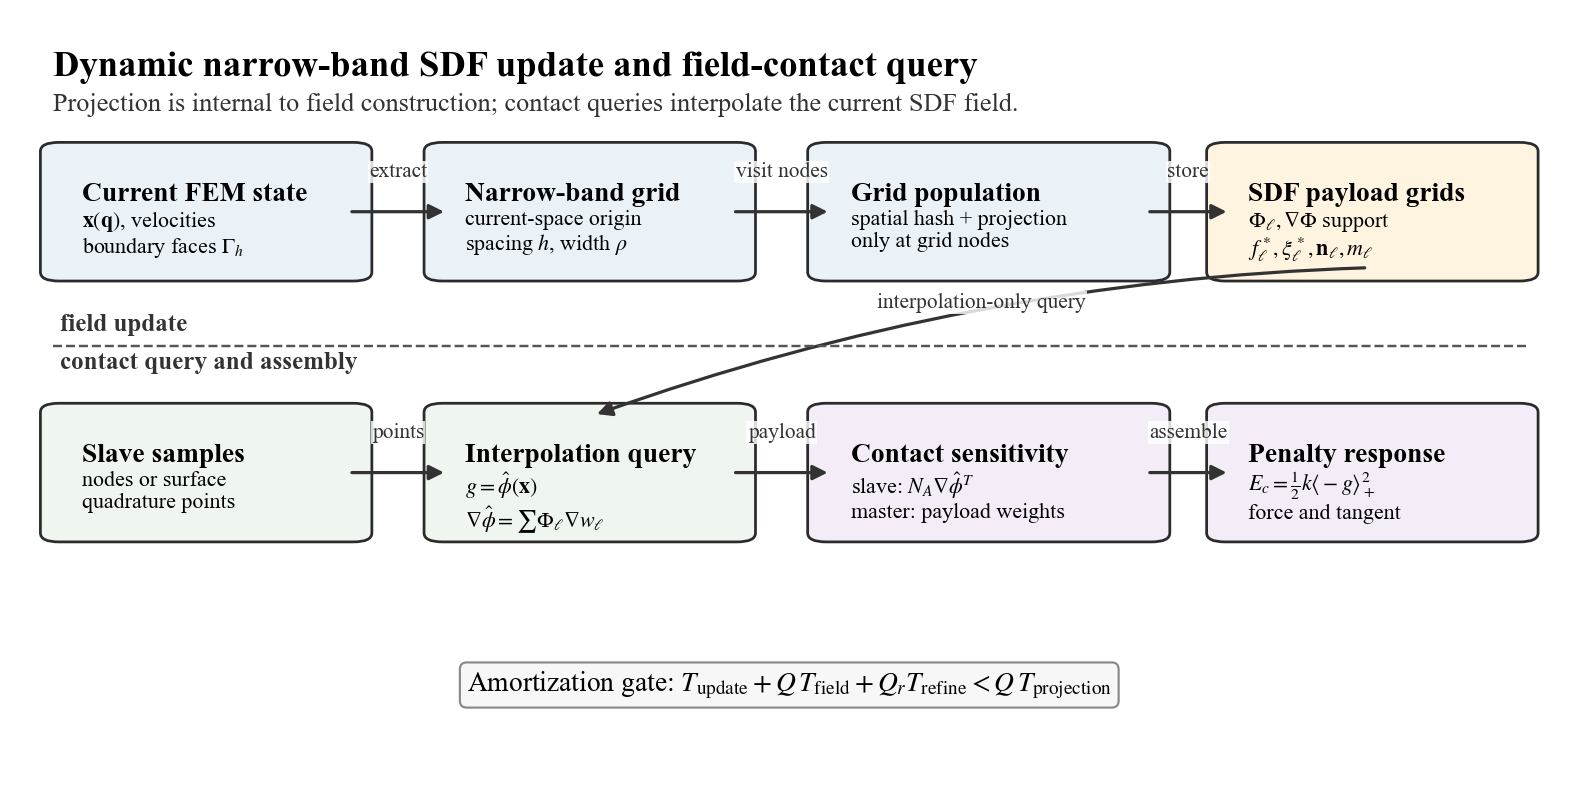
\includegraphics[width=0.98\linewidth]{dynamic_sdf_method_schematic.png}

\parbox{0.94\linewidth}{\small Figure~\thefigure: Compact architecture of the dynamic narrow-band SDF update and field-contact query. The upper row is the current-configuration field update, where projection is used only to populate grid-node values and closest-feature payloads. The lower row is the repeated contact path, which evaluates gaps, scalar-field derivatives, Jacobians, and penalty forces by interpolation.}
\end{center}

Valid grid nodes are populated by an internal spatial-hash projection kernel. For each valid node, the kernel searches nearby current boundary triangles, computes the signed closest distance, and stores the distance value, closest face id, barycentric coordinates, and closest-feature normal. This projection work is part of \(T_\mathrm{update}\), not part of the repeated query cost. After population, the query path is restricted to trilinear interpolation of \(\Phi_\ell\) and the payload grids. Out-of-band or invalid interpolation cells are rejected rather than silently falling back to projection; projection can reappear only when an explicit refinement mode is requested.

\section{Field-Interpolated Contact Formulation}

For a slave sample point
\begin{equation}
\mathbf{x}_i^A =
\sum_{b\in I_A} N_b^A \mathbf{x}_b^A ,
\end{equation}
the contact gap is the trilinearly interpolated SDF:
\begin{equation}
g_i =
\hat{\phi}_B(\mathbf{x}_i^A)
=
\sum_{\ell\in\mathcal{C}(\mathbf{x}_i^A)}
w_\ell(\mathbf{x}_i^A)\Phi_\ell .
\end{equation}
The spatial derivative used by the slave Jacobian is the analytic derivative of this scalar interpolation:
\begin{equation}
\nabla_x\hat{\phi}_B(\mathbf{x}_i^A)
=
\sum_{\ell\in\mathcal{C}(\mathbf{x}_i^A)}
\Phi_\ell\,\nabla_x w_\ell(\mathbf{x}_i^A) .
\end{equation}
The contact normal is the normalized scalar-field derivative,
\begin{equation}
\mathbf{n}_i =
\frac{\nabla_x\hat{\phi}_B(\mathbf{x}_i^A)}
{\|\nabla_x\hat{\phi}_B(\mathbf{x}_i^A)\|}.
\end{equation}
An interpolated closest-feature normal \(\tilde{\mathbf{n}}_i=\mathrm{normalize}(\sum_\ell w_\ell \mathbf{n}_\ell)\) is retained only as a geometric normal estimate for diagnostics or explicit refinement; it is not the derivative of the scalar gap.
The sign convention is positive for separation and negative for penetration.

The slave Jacobian is
\begin{equation}
\frac{\partial g_i}{\partial \mathbf{x}_b^A}
=
N_b^A \nabla_x\hat{\phi}_B(\mathbf{x}_i^A)^T .
\end{equation}
The master Jacobian is assembled from the interpolated closest-feature payload:
\begin{equation}
\frac{\partial g_i}{\partial \mathbf{x}_a^B}
=
-
\sum_{\ell\in\mathcal{C}(\mathbf{x}_i^A)}
w_\ell(\mathbf{x}_i^A)
N_a^\Gamma(\boldsymbol{\xi}_\ell^\ast)
\mathbf{n}_\ell^T .
\end{equation}

For frictionless normal penalty contact,
\begin{equation}
E_c =
\frac{1}{2}k\langle -g_i\rangle_+^2,
\qquad
\lambda_i =
k\langle -g_i\rangle_+,
\qquad
\mathbf{f}_{c,i} =
\mathbf{J}_i^T\lambda_i .
\end{equation}
A Gauss-Newton contact stiffness approximation is assembled as \(k\mathbf{J}_i^T\mathbf{J}_i\).

\section{Algorithm and Cost Model}

One update/query cycle extracts current boundary triangles, builds \(\mathcal{G}_\rho(\Gamma_h)\), populates grid-node distance and payload values with the projection kernel, evaluates contact samples by interpolation, differentiates the scalar interpolation for slave sensitivities, and assembles field-contact Jacobians and penalty forces. Algorithm~1 summarizes the update and assembly sequence used in the implementation.

\begin{center}
\small
\textbf{Algorithm 1. Dynamic narrow-band SDF update and field-contact assembly.}
\vspace{0.4em}

\renewcommand{\arraystretch}{1.08}
\begin{tabular}{p{0.94\linewidth}}
\toprule
\textbf{Algorithm 1: Current-space dynamic SDF field contact} \\
\midrule
\textbf{Input:} master nodal positions \(\mathbf{x}^B\), boundary faces \(F^B\), slave samples \(S^A\), spacing \(h\), band width \(\rho\), penalty \(k\). \\
1. Extract the current master surface \(\Gamma_h^B(\mathbf{q})\) and oriented boundary normals from \((\mathbf{x}^B,F^B)\). \\
2. Build an inflated current-space grid \(\mathcal{G}_\rho\), including any required padding for candidate slave interpolation cells. \\
3. Mark grid nodes inside the narrow band; reject nodes outside the validity mask. \\
4. For each valid node \(\mathbf{y}_\ell\), use the spatial-hash projection kernel to store \(\Phi_\ell\), \(f_\ell^\ast\), \(\boldsymbol{\xi}_\ell^\ast\), \(\mathbf{n}_\ell\), and \(m_\ell\). \\
5. For each slave sample \(\mathbf{x}_i^A\in S^A\), compute \(g_i=\sum_\ell w_\ell\Phi_\ell\) and \(\nabla_x\hat{\phi}_i=\sum_\ell\Phi_\ell\nabla_x w_\ell\) by interpolation only. \\
6. If \(g_i<0\), assemble \(J_A=N_A\nabla_x\hat{\phi}_i^T\) and \(J_B=-\sum_\ell w_\ell N^\Gamma(\boldsymbol{\xi}_\ell^\ast)\mathbf{n}_\ell^T\). \\
7. Accumulate \(\lambda_i=k\langle -g_i\rangle_+\), contact force \(\mathbf{J}_i^T\lambda_i\), optional Gauss--Newton stiffness, and update/query timings. \\
\textbf{Output:} dynamic SDF field, field-contact residuals/Jacobians, and \(T_\mathrm{update}\), \(T_\mathrm{field}\), \(T_\mathrm{refine}\) if refinement is enabled. \\
\bottomrule
\end{tabular}
\end{center}

The field is beneficial only when the update cost is amortized over enough queries. With optional refinement count \(Q_r\), the measured gate is
\begin{equation}
T_\mathrm{update}
+
Q T_\mathrm{field}
+
Q_r T_\mathrm{refine}
<
Q T_\mathrm{projection}.
\end{equation}
Without refinement,
\begin{equation}
Q^\ast =
\frac{T_\mathrm{update}}
{T_\mathrm{projection}-T_\mathrm{field}} .
\end{equation}
The paper therefore claims acceleration only for query counts exceeding the measured crossover \(Q^\ast\).

\section{Implementation}

The field implementation is in \path{src/sfc/sdf/narrow_band_grid.py} and \path{src/sfc/sdf/dynamic_narrow_band_sdf.py}. The query API includes \path{query_phi} and \path{query_spatial_derivative_phi}; \path{query_gradient} is the derivative of the scalar \(\phi\) interpolation, while \path{query_geometric_normal} exposes the optional interpolated closest-feature normal. The field-contact implementation is in \path{src/sfc/contact/field_contact.py}. It contains a preserved \path{node_to_surface_field_penalty_response} path for node/sample contact, a reference \path{surface_to_surface_field_penalty_response} path for triangle quadrature, and a vectorized surface-to-surface response used for the paper-facing CalculiX native-contact comparisons. The older projection path in \path{src/sfc/sdf/dynamic_surface_sdf.py} is retained as \path{surface_projection_distance_kernel} for field construction, validation references, and explicitly requested refinement.

The core finite-element mechanics remain internally assembled and independent of Abaqus-generated matrices, force files, \texttt{.odb} files, and spreadsheet outputs. No friction, self-contact, nonlinear FEM main method, GPU path, barrier contact, POD, neural SDF, or Abaqus dependency is introduced.

\section{Experiments}

The primary SDF-field outputs are generated by:
\begin{quote}
\footnotesize\ttfamily
python validation/run\_true\_dynamic\_sdf\_field\_validation.py\\
--out-dir results/true\_sdf\_final
\end{quote}
The experiment uses a deterministic nonplanar triangulated current surface with 512 triangles and three grid spacings. The query path is interpolation-only; projection appears only in field construction and reference/error measurement. All reported gradient and Eikonal quantities use \(\sum_\ell\Phi_\ell\nabla_x w_\ell\), the derivative of the scalar gap interpolation.

\subsection{SDF Field Accuracy}

This experiment evaluates whether the rebuilt current-space field remains a usable local SDF as grid spacing changes. The reference distance and normal are computed by projecting each sample to the current triangulated surface, while the method evaluates the same samples by field interpolation. Table~\ref{tab:field-accuracy} shows that the scalar gap error decreases as the spacing is refined; the normal error remains bounded because it is computed from the piecewise trilinear scalar derivative on a triangulated nonplanar surface.

\begin{table}[t]
\centering
\small
\caption{Dynamic narrow-band SDF field accuracy on the nonplanar current surface.}
\label{tab:field-accuracy}
\begin{tabular}{rrrrrr}
\toprule
Spacing & Grid nodes & Valid nodes & Max \(\phi\) error & Max normal error & Max Eikonal residual \\
\midrule
0.100 & 1792 & 876 & \(1.835893\times10^{-3}\) & \(5.751473\times10^{-2}\) & \(6.784055\times10^{-3}\) \\
0.075 & 3969 & 2174 & \(1.132281\times10^{-3}\) & \(4.769023\times10^{-2}\) & \(4.546733\times10^{-3}\) \\
0.050 & 12493 & 7826 & \(5.114950\times10^{-4}\) & \(3.600289\times10^{-2}\) & \(4.743522\times10^{-3}\) \\
\bottomrule
\end{tabular}
\end{table}

\begin{figure}[t]
  \centering
  \includegraphics[width=0.72\linewidth]{field_phi_error_vs_spacing.png}
  \caption{Field \(\phi\) error decreases with grid spacing for the tested nonplanar surface.}
\end{figure}

\begin{figure}[t]
  \centering
  \includegraphics[width=0.72\linewidth]{field_eikonal_residual_vs_spacing.png}
  \caption{Maximum Eikonal residual over the dynamic narrow band.}
\end{figure}

\subsection{Jacobian Finite-Difference Check}

This experiment checks whether the field-contact Jacobian is actually the derivative of the field gap used in the penalty energy. The slave block is compared against finite differences of \(\hat{\phi}(\mathbf{x})\), and the master block is compared against finite differences after rebuilding the field under master nodal perturbations. The small errors in Table~\ref{tab:field-jacobian} verify both the scalar-interpolation derivative used on the slave side and the closest-feature payload sensitivity used on the master side.

\begin{table}[t]
\centering
\small
\caption{Field-contact Jacobian finite-difference check.}
\label{tab:field-jacobian}
\begin{tabular}{lrrrr}
\toprule
Case & Gap & Slave FD error & Master FD error & Status \\
\midrule
single slave / large triangle & \(-1.30\times10^{-1}\) & \(2.875566\times10^{-11}\) & \(1.462164\times10^{-11}\) & passed \\
\bottomrule
\end{tabular}
\end{table}

\begin{figure}[t]
  \centering
  \includegraphics[width=0.62\linewidth]{field_contact_jacobian_fd_error.png}
  \caption{Slave and master field-contact Jacobian finite-difference errors.}
\end{figure}

\paragraph{Current-space SDF sanity check.}

This experiment isolates why a current-space field is needed for deformable FEM contact. The baseline keeps a frozen material-space plane SDF and evaluates it after tilt or shear deformation, while the proposed field is rebuilt from the current surface. The material-space field accumulates gap and normal errors because it no longer represents the deformed boundary; the rebuilt dynamic field avoids this mismatch.

\begin{table}[t]
\centering
\small
\caption{Frozen material-space SDF compared with the rebuilt dynamic field.}
\label{tab:material-baseline}
\begin{tabular}{lrrrr}
\toprule
Case & Dynamic \(\phi\) err. & Dynamic normal err. & Material \(\phi\) err. & Material normal err. \\
\midrule
tilt\_x & \(8.326673\times10^{-17}\) & \(1.523921\times10^{-15}\) & \(9.783015\times10^{-2}\) & \(1.193580\times10^{-1}\) \\
shear\_xy & \(5.551115\times10^{-17}\) & \(3.351421\times10^{-15}\) & \(4.265482\times10^{-2}\) & \(9.962740\times10^{-2}\) \\
\bottomrule
\end{tabular}
\end{table}

\begin{figure}[t]
  \centering
  \includegraphics[width=0.72\linewidth]{material_space_vs_dynamic_field_error.png}
  \caption{Material-space SDF error under current-surface deformation compared with the rebuilt dynamic field.}
\end{figure}

\subsection{Amortized Timing and Crossover}

The dynamic field is not claimed to be faster for small query counts. Its update cost is paid once per rebuild, while the interpolation query cost is paid per contact sample. Table~\ref{tab:timing} reports the measured crossover \(Q^\ast\): finer spacing improves field resolution but increases update cost, so \(Q^\ast\) rises from hundreds to several thousand queries.

\begin{table}[t]
\centering
\small
\caption{Update/query timing and measured crossover count. Times are seconds.}
\label{tab:timing}
\begin{tabular}{rrrrrr}
\toprule
Spacing & \(T_\mathrm{update}\) & \(T_\mathrm{field}\) & \(T_\mathrm{projection}\) & \(T_\mathrm{refine}\) & \(Q^\ast\) \\
\midrule
0.100 & 14.330253 & \(5.626483\times10^{-5}\) & \(1.749774\times10^{-2}\) & \(5.731850\times10^{-4}\) & 822 \\
0.075 & 29.062764 & \(5.340050\times10^{-5}\) & \(1.747250\times10^{-2}\) & \(5.369825\times10^{-4}\) & 1669 \\
0.050 & 78.940208 & \(5.365200\times10^{-5}\) & \(1.742862\times10^{-2}\) & \(4.956188\times10^{-4}\) & 4544 \\
\bottomrule
\end{tabular}
\end{table}

The field acceleration claim is supported only for \(Q>Q^\ast\) under the measured inequality. Optional refinement is implemented and timed, but the main acceleration gate uses \(Q_r=0\).

\begin{figure}[t]
  \centering
  \includegraphics[width=0.72\linewidth]{field_timing_components.png}
  \caption{Field update, field query, and projection query timing components.}
\end{figure}

\begin{figure}[t]
  \centering
  \includegraphics[width=0.72\linewidth]{field_speedup_vs_query_count.png}
  \caption{Amortized speedup as projection-query total time divided by SDF-field total time. Dashed vertical markers indicate measured crossover counts.}
\end{figure}

\begin{figure}[t]
  \centering
  \includegraphics[width=0.72\linewidth]{field_crossover_qstar.png}
  \caption{Measured crossover query count \(Q^\ast\) for each grid spacing.}
\end{figure}

\subsection{Quasi-Static Multi-Step Native Contact}

We compare the independent SFC true-field contact solve against CalculiX native surface-to-surface contact on three benchmark-style quasi-static geometries. CalculiX receives its own \texttt{*CONTACT PAIR} model and SFC independently solves the corresponding \path{DynamicNarrowBandSDF + field_contact} model; the comparison is not a replay and does not use CalculiX inside the core SDF path. Each case now uses 21 closure/load steps. Because the first V-indenter step has a nearly zero reference displacement, pointwise relative error is denominator-limited; the plotted evidence therefore reports full-curve displacement \(L^2\) error, while Table~\ref{tab:native-contact} reports nonzero-load maxima for stress-like fields.

\begin{table}[t]
\centering
\tiny
\setlength{\tabcolsep}{2pt}
\caption{Independent CalculiX native contact versus SFC dynamic-SDF contact over 21 quasi-static closure/load steps. Times are wall-clock seconds for the tested Python/CalculiX runs.}
\label{tab:native-contact}
\begin{tabular}{lrrrrrrr}
\toprule
Problem & Curve disp. err. & Max strain err. & Max stress err. & Max VM err. & SFC & CCX & CCX/SFC \\
\midrule
sphere indentation & \(2.761745\times10^{-3}\) & \(4.521653\times10^{-2}\) & \(4.346932\times10^{-2}\) & \(4.415077\times10^{-2}\) & 11.137 & 13.633 & 1.224 \\
V-indenter & \(7.056039\times10^{-3}\) & \(6.728597\times10^{-2}\) & \(6.477352\times10^{-2}\) & \(6.297838\times10^{-2}\) & 3.371 & 14.106 & 4.185 \\
cylinder compression & \(4.502934\times10^{-4}\) & \(2.190308\times10^{-3}\) & \(1.723906\times10^{-3}\) & \(1.291308\times10^{-3}\) & 69.291 & 48.107 & 0.694 \\
\bottomrule
\end{tabular}
\end{table}

\begin{figure}[t]
  \centering
  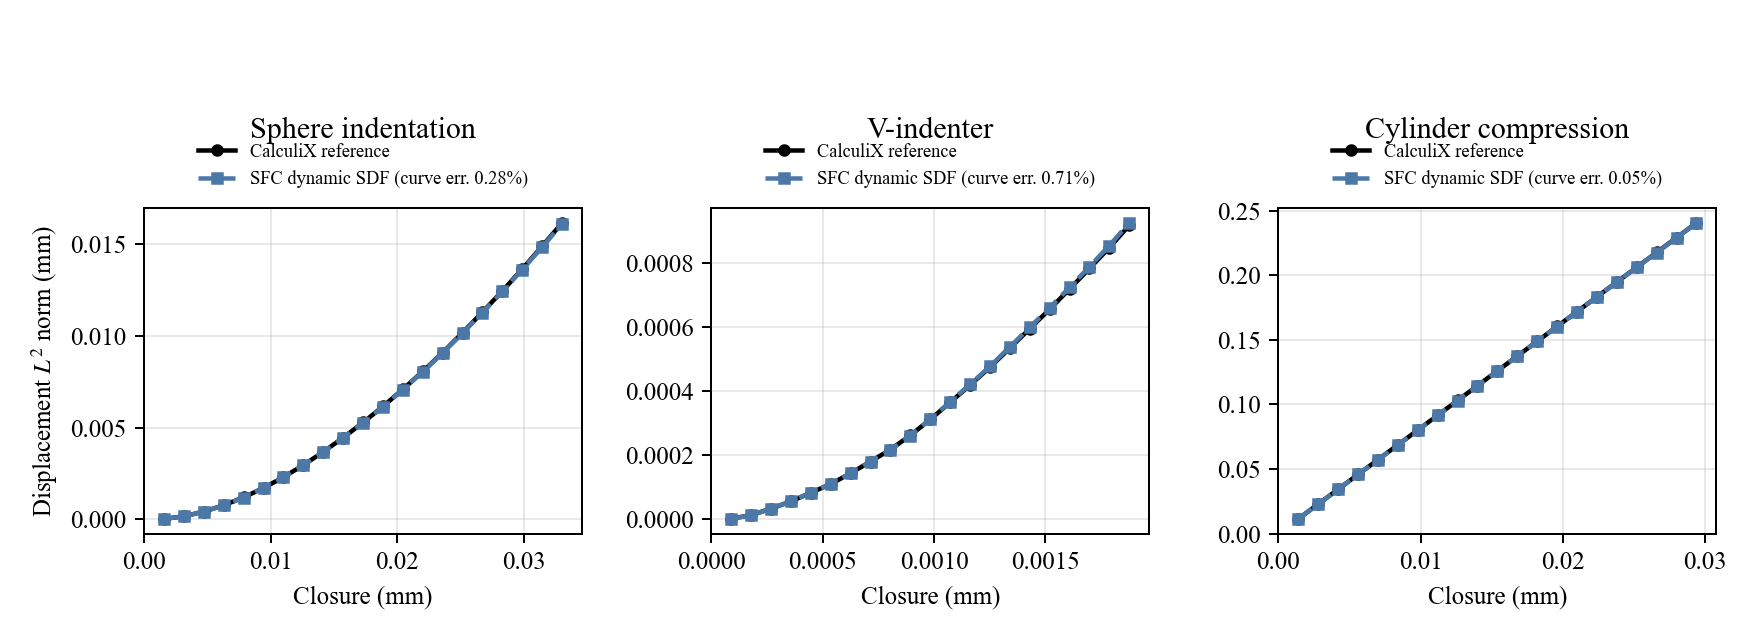
\includegraphics[width=0.96\linewidth]{native_contact_displacement_curves.png}
  \caption{Quasi-static closure/load displacement-norm trajectories for independent CalculiX native contact and SFC dynamic-SDF contact. Each case uses 21 closure steps, and each SFC legend reports the full-curve displacement \(L^2\) relative error.}
\end{figure}

\subsection{Three-Second C3D8 Dynamic Time History}

The dynamic case uses a deformable C3D8 block contacting a deformable C3D8 master block through the true field-contact path for three seconds of physical time. The runner exports \(z\)-displacement, normal force, contact energy, minimum gap, and active contact sample histories at 151 time points. The fine-grid cloud is taken at the peak normal-force state so that the displacement, strain, stress, gap, pressure, and active-contact fields are visually auditable.

\begin{figure}[t]
  \centering
  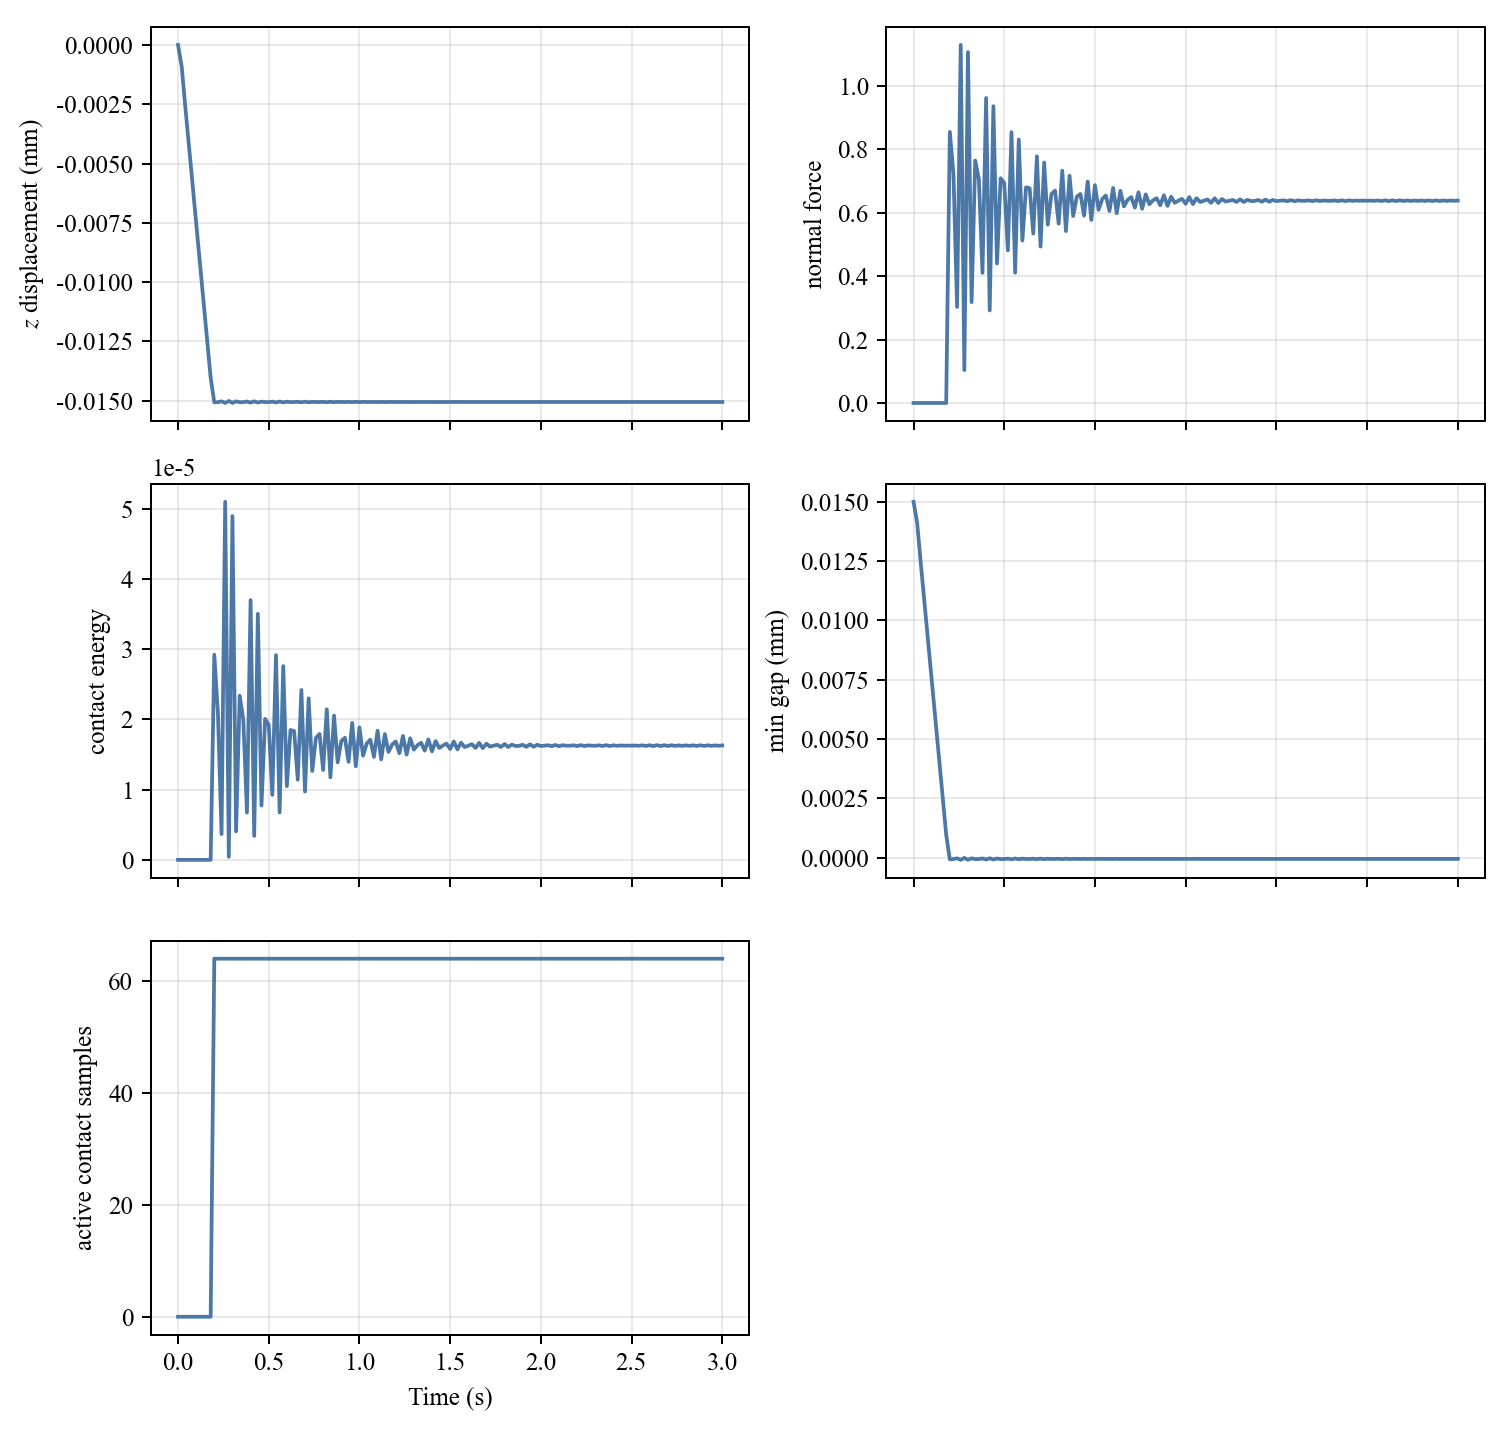
\includegraphics[width=0.88\linewidth]{long_time_c3d8_dynamic_histories.png}
  \caption{Three-second C3D8 dynamic SDF-contact time histories. The horizontal axis is physical time; the outputs are \(z\)-displacement, normal force, contact energy, minimum gap, and active contact sample count.}
\end{figure}

\begin{figure}[t]
  \centering
  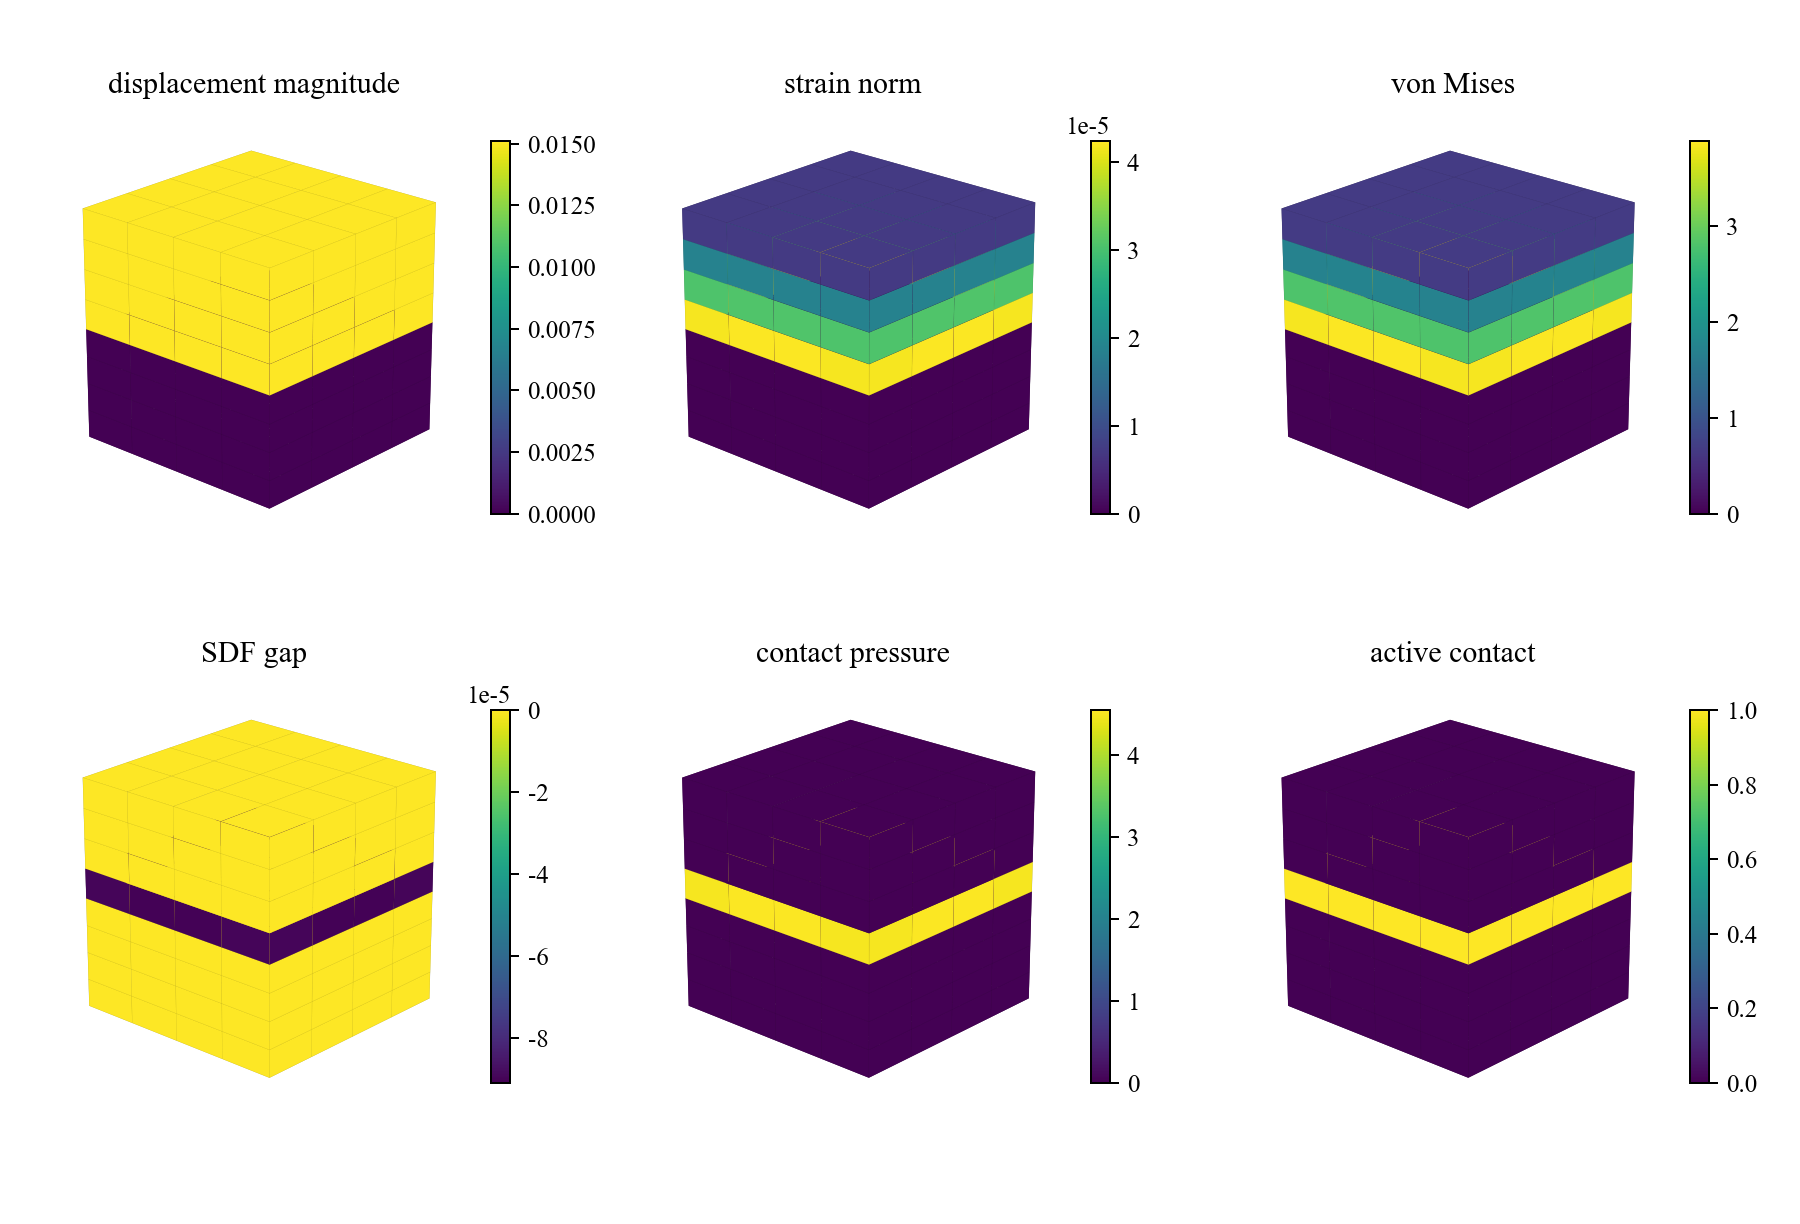
\includegraphics[width=0.92\linewidth]{fine_grid_c3d8_contact_clouds.png}
  \caption{Fine-grid C3D8 dynamic contact cloud at the peak normal-force state: displacement magnitude, strain norm, von Mises stress, SDF gap, contact pressure, and active contact mask.}
\end{figure}

\subsection{Fig. 6-Inspired Complex Frictionless Contact}

To add a more engineering-like visual contact case without importing a frictional stick-slip claim, we build a Fig.~6-inspired configuration: a \(20\times10\times2\) mm lower C3D8 block and a \(4.5\times4.5\) mm upper rectangular driver. The driver first applies normal closure and then a lateral offset while the contact law remains frictionless. The resulting field solve uses a \(24\times12\times4\) C3D8 lower mesh, a true current-space narrow-band SDF on the lower surface, and seven-point surface quadrature on the driver. The final shifted stage reaches a minimum gap of \(-2.92\times10^{-2}\) mm with 672 active quadrature samples.

\begin{figure}[t]
  \centering
  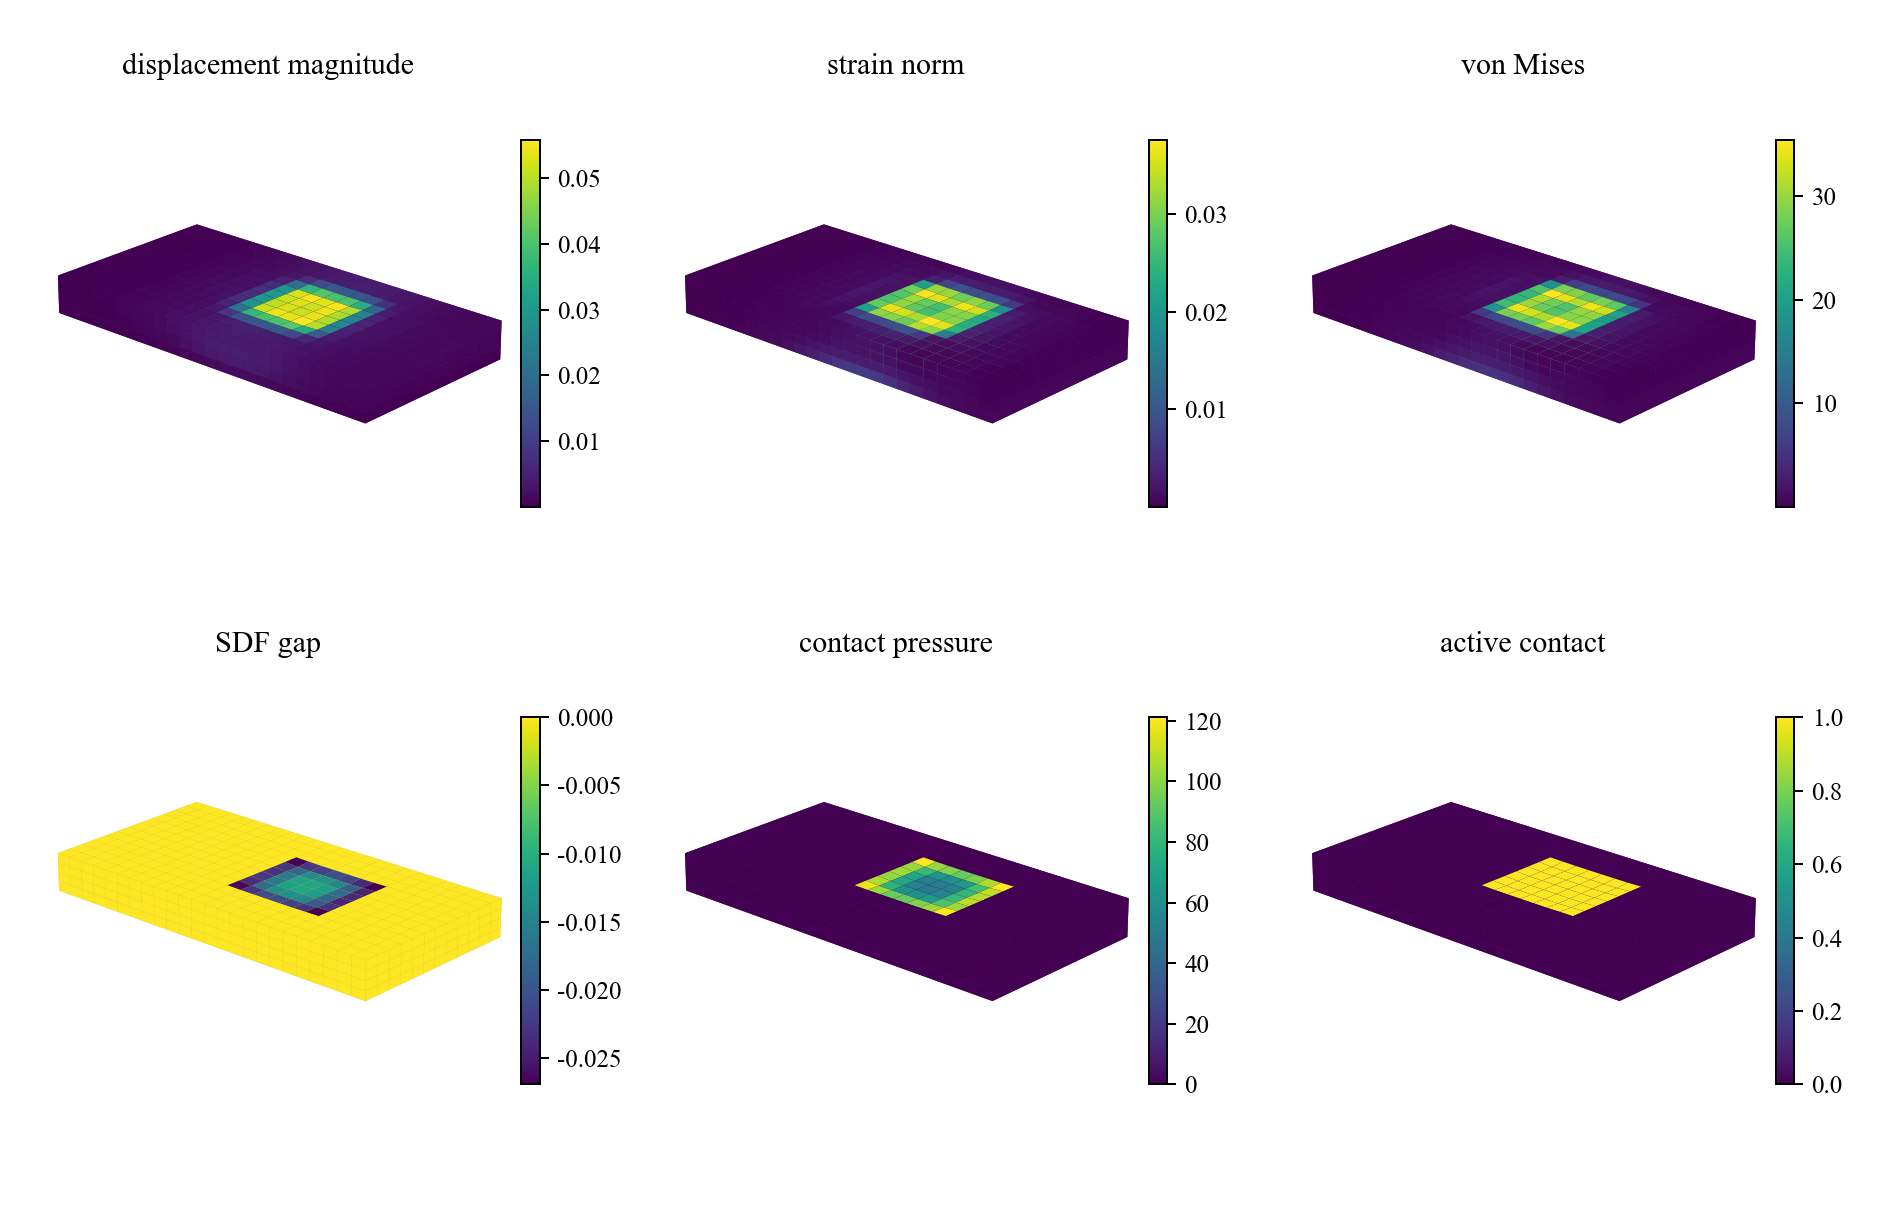
\includegraphics[width=0.92\linewidth]{fig6_inspired_shifted_frictionless_clouds.png}
  \caption{Fig.~6-inspired frictionless complex contact cloud for the shifted loading stage. The panels show three-dimensional displacement, strain, von Mises stress, SDF gap, contact pressure, and active-contact mask fields.}
\end{figure}

\begin{figure}[t]
  \centering
  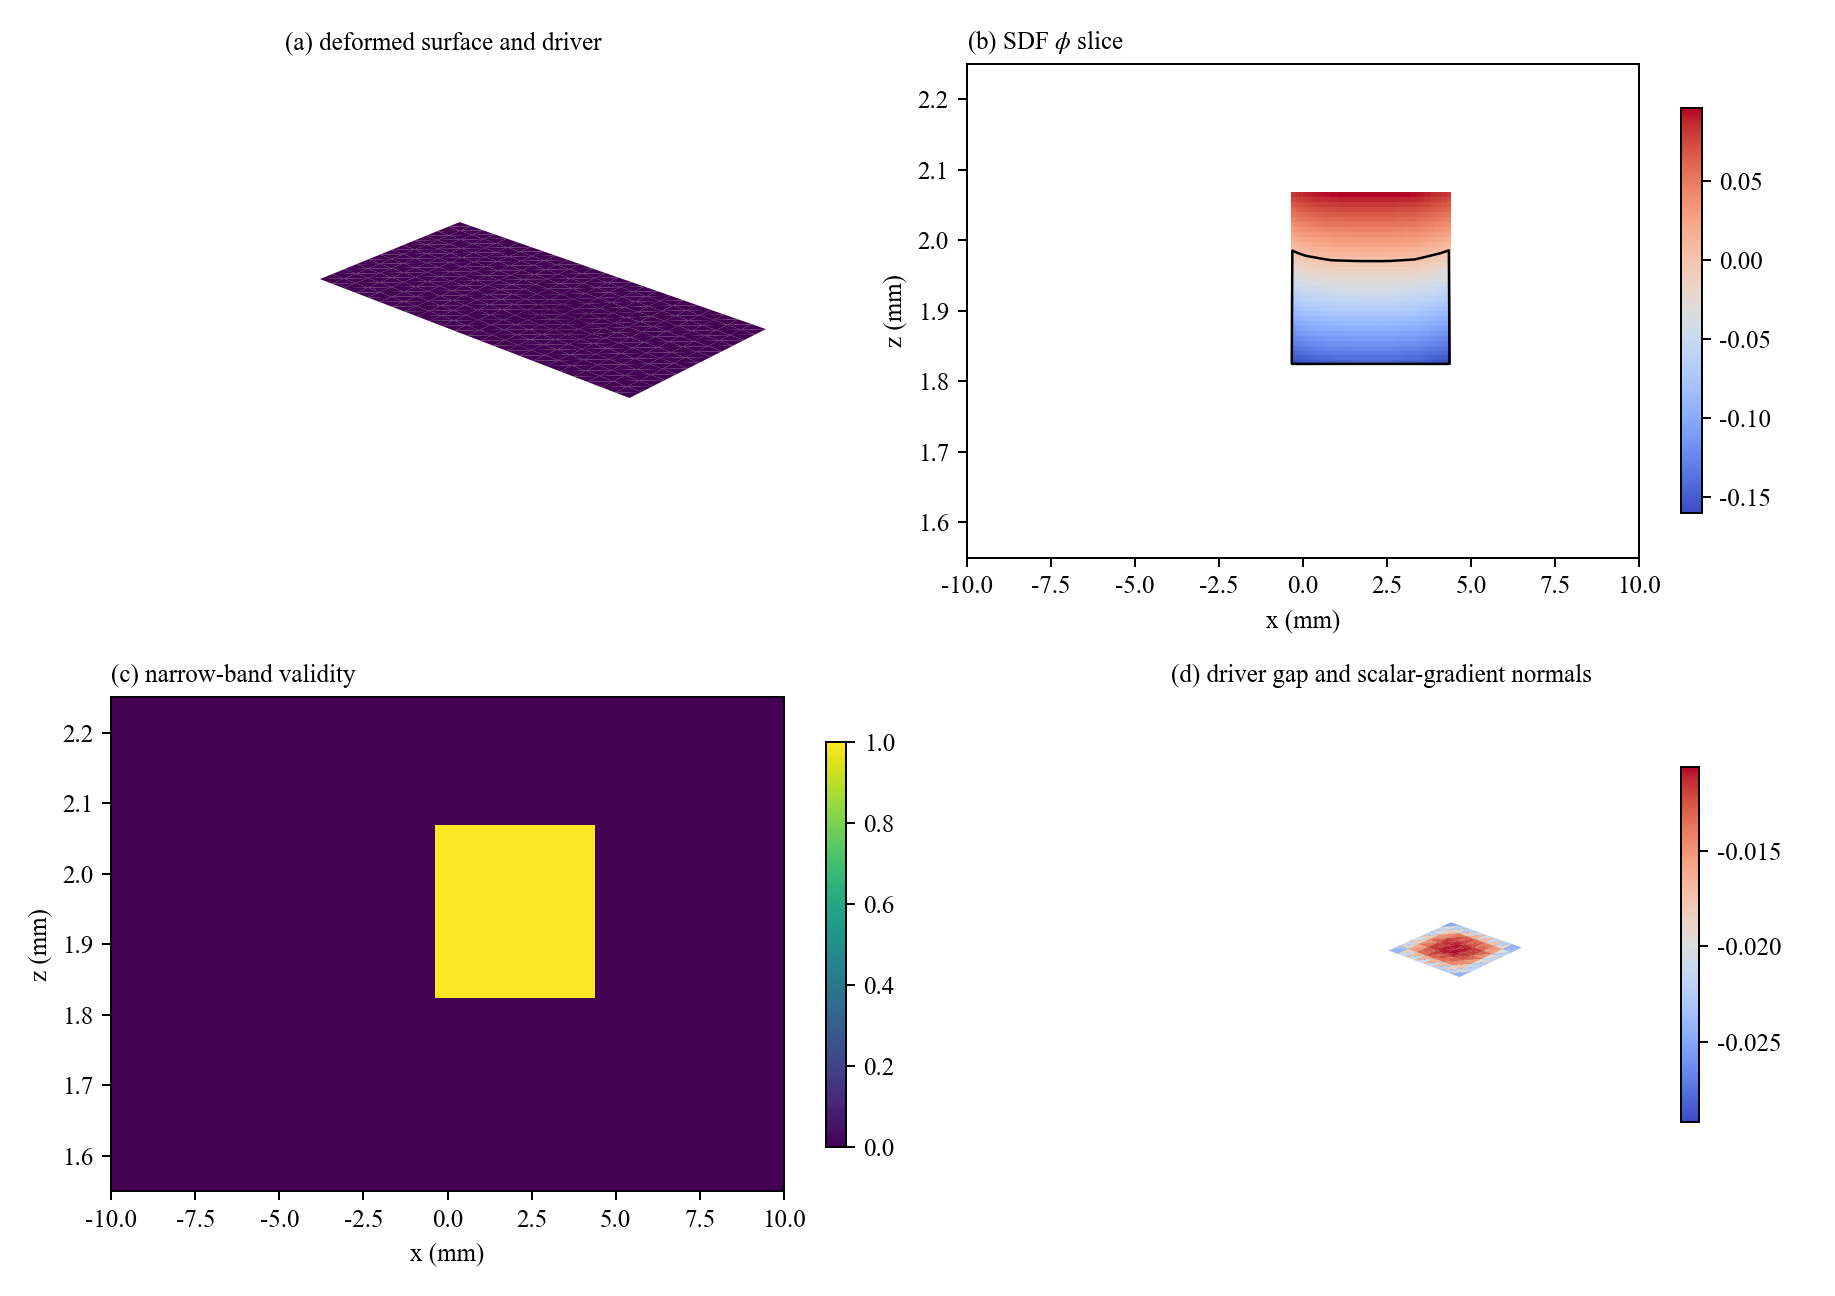
\includegraphics[width=0.92\linewidth]{fig6_inspired_sdf_field_visualization.png}
  \caption{SDF-field visualization for the Fig.~6-inspired case: deformed contact surface and driver, \(\phi\) slice with zero contour, narrow-band validity, and driver gap with scalar-gradient normals.}
\end{figure}

\subsection{Backend and Timing Ablation}

The field-query crossover is also reflected at the step level in contact-dominated TET4/HEX8 static and dynamic tests. These tests compare the true-field path against the spatial-hash projection timing reference while keeping the gap and force agreement at numerical roundoff. The field path is faster in all 16 non-quick rows, with measured projection/field step speedups from \(7.51\times\) to \(24.17\times\) and a minimum measured query crossover of \(24.61\) samples for the tested workload.

\begin{figure}[t]
  \centering
  \includegraphics[width=0.92\linewidth]{solver_step_timing_breakdown.png}
  \caption{Solver-level timing breakdown for TET4/HEX8 static and dynamic contact-dominated workloads. Diamonds mark the projection-reference total step time.}
\end{figure}

\begin{figure}[t]
  \centering
  \includegraphics[width=0.92\linewidth]{solver_step_speedup.png}
  \caption{Projection-reference total step time divided by true-field total step time for the solver-level timing cases.}
\end{figure}

Finally, an 11-step reduced-mesh backend ablation separates the preserved node-to-surface path from the surface-to-surface implementations. The non-vectorized surface-to-surface path is a correctness reference; the vectorized path preserves the same endpoint metrics while reducing the quadrature/contact query cost from 14.58 s to 0.061 s in this representative run. Forced spatial-hash grouped field construction is retained for larger candidate sets, although it is slower on this small ablation because grouping overhead dominates.

\begin{figure}[t]
  \centering
  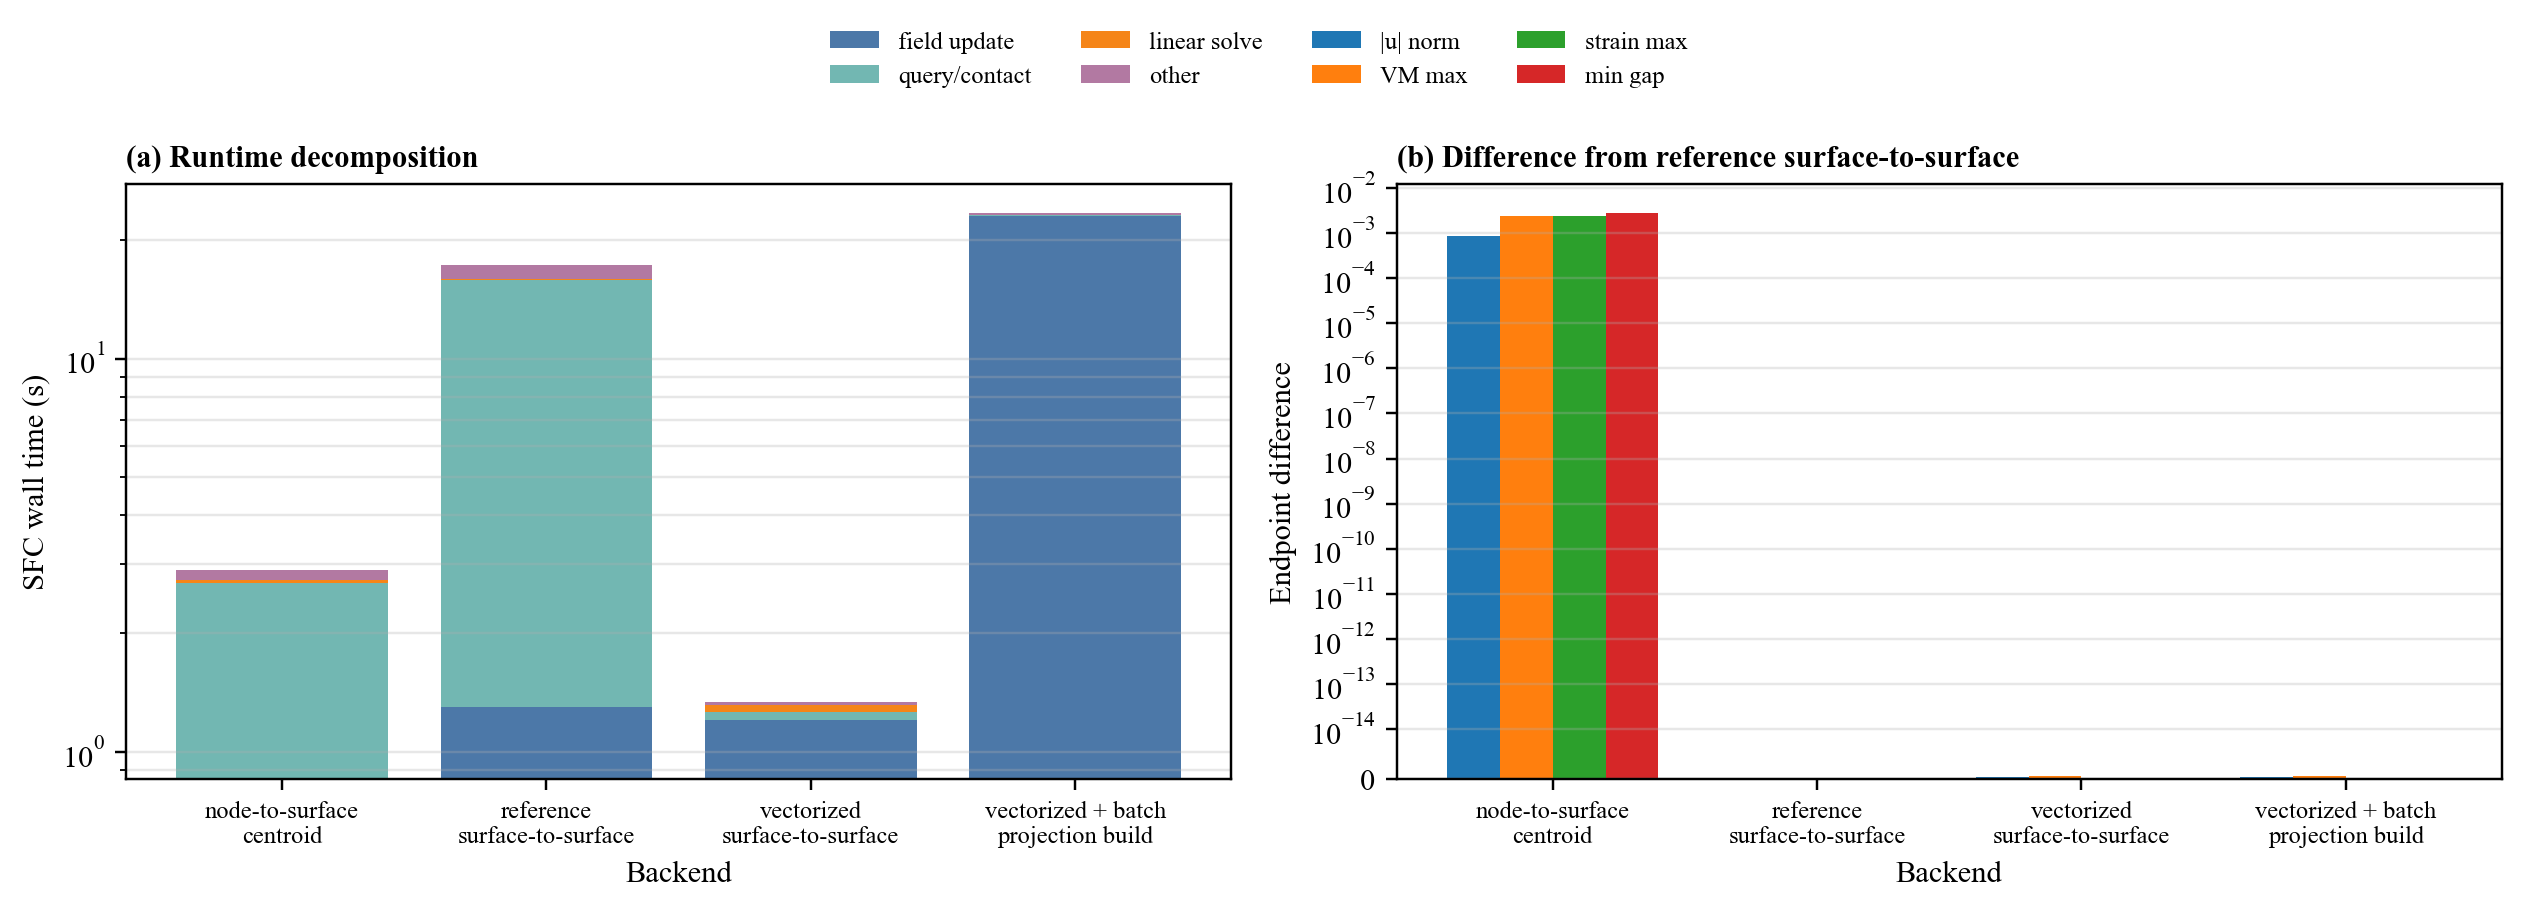
\includegraphics[width=0.96\linewidth]{backend_ablation_overview.png}
  \caption{Representative backend ablation for node-to-surface sampling, reference surface-to-surface quadrature, vectorized surface-to-surface quadrature, and vectorized field contact with forced batch projection during field construction. The legend is placed outside the axes so the timing bars and endpoint-difference bars remain unobstructed.}
\end{figure}

\FloatBarrier

\section{Scope of Claims}

The reported experiments support true dynamic narrow-band SDF field existence, interpolation-only query, field accuracy under the reported thresholds, slave/master field-contact Jacobian finite-difference consistency, 21-step quasi-static native-contact agreement, three-second C3D8 dynamic field-contact histories, and SDF acceleration after the measured \(Q^\ast\) crossover. The solver-level tests support the scoped statement that the optimized true-field backend can reduce contact-dominated TET4/HEX8 step time after the measured crossover, while the backend ablation documents both node-to-surface and surface-to-surface integration paths.

The Fig.~6-inspired case supports physical auditability of displacement, strain, stress, gap, pressure, active-contact, and SDF-field visualizations in a more engineering-like geometry. It is not evidence for frictional stick-slip, and it is not used to prove the SDF acceleration claim.

The current results do not support claims of robust global SDF behavior for arbitrary non-manifold geometry, friction, self-contact, nonlinear FEM as the main method, GPU acceleration, barrier contact, superiority over production BVH, or Abaqus-dependent core solver behavior.

\section{Supplementary Context}

Additional CalculiX, C3D8, SfePy, and external-solver replay results are not the main evidence for this method. They may be retained as supplementary context for external deformed-state checks, but the main paper claims are field construction, field interpolation, field-contact Jacobians, penalty force assembly, native FEM-SDF contact trajectories, and amortized SDF update/query cost.

\section{Limitations}

The field is valid only in the constructed narrow band. Sign handling assumes consistently oriented current surfaces in the tested cases. The current paper-facing implementation targets internally assembled linear finite-element mechanics and frictionless normal penalty contact. Timing results are Python prototype measurements and should not be interpreted as production BVH or hardware acceleration claims.

\section{Conclusion}

This paper presented a training-free dynamic narrow-band SDF field for finite-element contact. The key distinction from projection-query contact is that closest-point projection is internalized as a field construction kernel, while repeated contact evaluation is performed by interpolation of \(\Phi_\ell\) and closest-feature payloads. The slave sensitivity is the analytic derivative of the scalar SDF interpolation, and the master sensitivity is assembled from closest-feature payloads. The experiments show field accuracy, Eikonal consistency, finite-difference Jacobian agreement, quasi-static and dynamic FEM-SDF contact trajectories, engineering-style three-dimensional contact clouds, and measured crossover counts for amortized acceleration.

\section*{Data Availability}

The scripts and tabulated numerical data used for the reported validation studies are available from the corresponding author upon reasonable request. A public archival repository can be linked at submission if required by the journal or funding body.

\section*{Declaration of Competing Interest}

The authors declare that they have no known competing financial interests or personal relationships that could have appeared to influence the work reported in this paper.

\section*{Funding}

This research did not receive any specific grant from funding agencies in the public, commercial, or not-for-profit sectors.

\section*{Declaration of Generative AI and AI-Assisted Technologies in the Manuscript Preparation Process}

During the preparation of this work, the authors used OpenAI Codex to support manuscript organization, consistency checks, and language revision. After using this tool, the authors reviewed and edited the content as needed and take full responsibility for the content of the published article.

\bibliographystyle{unsrt}
\bibliography{references}

\end{document}
